\section{Empirical Action-Class Risk and Semantic Preference}
\label{sec:pending-studies}
The follow-up connects the class-risk theorem to the retained representations and evaluates transport under a new language construction. Its original five analyses completed without dropping declared conditions: 48 spectral cells, 48 constructed witnesses, all 2,952 image-subgroup units, 36 fixed mechanism settings, and 48 new-context cells. The methods and provenance are in \cref{app:pending-protocols}; the results below concern distinct targets rather than a pooled success score. We separately report the completed $16\!\to\!8$ spectral sensitivity check in \cref{app:spectral-dimension-sensitivity} and the same-bank independent-orthogonal comparison at both dimensions in \cref{app:orthogonal-results}.

\subsection{Risk magnitude, heterogeneity and constructed-action transfer}
\paragraph{Three evaluation targets.}
The finite-bank analysis uses the test bank's own second moment and describes the optimum on that complete bank. The construction check uses training whitening and verifies the constructed action against the theorem on the same construction bank. The held-out comparison then freezes both training whitening and fitted maps before scoring test representations. That test distribution need not have identity second moment in the training metric. The first target is descriptive structure, the second a same-bank construction check, and the third predictive transfer; none is substituted for another.

\begin{table}[H]
\caption{Finite-bank exact-action bounds in the test-bank metric. Each domain has 24 model/readout cells at $r=16$. The bounds concern cell-specific $L^\star$ over the entire exact orthogonal-action class in each test bank's own second-moment-whitened metric; displayed endpoints average those bounds, not confidence limits. $b_{\rm triv}$ is selected trivial-type energy divided by $r$. The last column counts unique highest-$\gamma_r$ ranks of the specified image among 120 C7 or three D4 images; it is not a rank of exact $L^\star$ or a significance test.}
\label{tab:followup-spectral}
\centering\small
\begin{tabular}{@{}lrrrrr@{}}
\toprule
Domain & Mean $\gamma_r$ & Mean bound endpoints & Mean $\eta$ & Mean $b_{\rm triv}$ & Image rank 1 \\
\midrule
$C_7$ & 0.98510 & [0.02980, 0.05863] & 0.02563 & 0.61540 & 7/24 \\
$D_4$ & 0.93528 & [0.12944, 0.24895] & 0.10321 & 0.72742 & 16/24 \\
\bottomrule
\end{tabular}
\end{table}

At the primary dimension $r=16$, the empirical spectral budget averages $0.98510$ for weekdays and $0.93528$ for corners. The corresponding mean cell-wise lower/upper bounds are $[0.02980,0.05863]$ and $[0.12944,0.24895]$ in the test bank's own second-moment-whitened metric (\cref{tab:followup-spectral}). These are deterministic bounds on the specified finite-bank action class. They establish compatibility at those risk levels, not existence of a native semantic computation.

Trivial-type components account for selected energy $b_{\rm triv}=0.61540/0.72742$ on average. Thus much of the retained budget is state-invariant, although a trivial component need not be purely contextual and a nontrivial component need not reflect computation. Here $b_{\rm triv}$ is selected energy divided by $r$, not total trivial energy $e_{\rm triv}$ or the fraction $b_{\rm triv}/\gamma_r$ of the selected budget. The real-type correction is at numerical scale in 47/48 conditions (absolute correction at most $5.33\times10^{-15}$). The exception is Llama-3.1-8B, C7, layer 13: $\Delta_{\rm type}=0.13235$, or $\Delta_{\rm type}/16=0.00827$. The typed restriction is essential to the theorem and counterexample, but changes this rank-16 panel materially in only one condition.

\begin{table}[t]
\centering\small
\begin{tabular}{@{}lrrrrr@{}}
\toprule
& Construction bank & \multicolumn{3}{c}{Old test bank, frozen training metric} & Witness worse \\
Domain & Witness & Witness & OLS & Ridge & than OLS \\
\midrule
$C_7$ & 0.02906 & 0.02806 & 0.02141 & 0.02141 & 24/24 \\
$D_4$ & 0.11996 & 0.11117 & 0.08878 & 0.08878 & 24/24 \\
\bottomrule
\end{tabular}
\caption{Transfer of frozen predictors at $r=16$ in the training metric. These means use training whitening for both construction and old test banks, including identity and fixed points. OLS and ridge need not obey group laws. The witness is feasible, not claimed optimal. Its transfer loss is not checked against Table~\ref{tab:followup-spectral}'s test-metric exact-orthogonal bounds: changing whitening can also change admissibility of the same raw-coordinate function (\cref{app:metric-conjugation}).}
\label{tab:followup-witness}
\end{table}

All 48 constructed witnesses satisfy the specified numerical action-law and orthogonality checks, and their construction-bank risks lie within the analytic bounds under those checks. With each witness constructed on training data and held fixed for testing, test losses average $0.02806/0.11117$, compared with $0.02141/0.08878$ for independent OLS (\cref{tab:followup-witness}). The witness is worse than OLS and fixed-coefficient ridge in every condition. Class inclusion ensures an optimal ordering on the same distribution and metric, not this ordering of training-fitted predictors on unseen data. The observed transfer ordering is therefore empirical; it concerns one constructor and does not establish that every exact action has worse held-out loss. The witness need not minimize $L^\star$. These prediction losses use \emph{training} whitening for both construction and test banks, whereas \cref{tab:followup-spectral} uses the test bank's own metric. The metrics also define different admissible classes of raw-coordinate functions. Conjugating the frozen training action into test-whitened coordinates preserves its group law but need not preserve orthogonality (\cref{app:metric-conjugation}); its transfer loss is therefore not checked against the test-bank exact-orthogonal bounds.

\begin{table}[t]
\centering\small
% Generated by analysis/main30_bounded_v1/derive.py; never edit numbers.
\begin{tabular}{lrrrr}
\toprule
Domain & Mean $\eta$ & Mean $L(I)$ & Mean $p^-$ & Mean $p^+$ \\
\midrule
C7 & 0.02563 & 0.76012 & 0.00416 & 0.03300 \\
D4 & 0.10321 & 0.52932 & 0.02624 & 0.14574 \\
\bottomrule
\end{tabular}

\caption{Same-metric reference and class-risk premium at $r=16$ on the original Study~2 test bank. Each domain averages \BoundedCellsPerDomain{} fixed cells equally. $p^-=\max\{0,2(1-\gamma_r)-\eta\}$ and $p^+=2(1-\gamma_r^2)-\eta$ are computed per cell before averaging. They bound the mean cost of imposing exact laws and orthogonality jointly. $L(I)$ uses total trivial energy and was also checked by direct residuals on the saved coordinates. These are finite-bank quantities, not transfer losses or confidence limits.}
\label{tab:bounded-risk}
\end{table}

\paragraph{The magnitude and concentration of the joint cost.}
\Cref{tab:bounded-risk} reports the same-metric identity reference and the bounds on $L^\star-\eta$ from \cref{eq:risk-premium-main}. The mean premium lies in $[\BoundedPremiumLowerCseven,\BoundedPremiumUpperCseven]$ for C7 and $[\BoundedPremiumLowerDfour,\BoundedPremiumUpperDfour]$ for D4. The lower-bound magnitudes are heterogeneous: median $p^-$ (range) is $0.000389$ ($[0.0000349,0.06254]$) for C7 and $0.01876$ ($[0.00254,0.08719]$) for D4; C7's unchanged equal-cell mean is strongly influenced by two cells (Llama-3.1-8B, layer 13, and Llama-3.2-3B, layer 11), which account for $90.7\%$ of its summed lower endpoints. All \BoundedAllPositive{} lower endpoints exceed the fixed numerical threshold $10^{-8}+10^{-7}|p^-|$ (\cref{app:bounded-risk-details}). Under the theorem assumptions, strict positivity already follows from $\eta>0$ (\cref{eq:positivity-main}); the information supplied here is its scale, heterogeneity and numerical separation from the fixed threshold. These lower endpoints concern exact laws and orthogonality jointly; the threshold is a software comparison rule, not a rigorous numerical-error bound or a significance test. Small lower endpoints do not show that the true premium is small, and the upper endpoints are bounds rather than measured optima. Identity risks average $\BoundedIdentityCseven/\BoundedIdentityDfour$, illustrating the gain available from state-dependent prediction even though much total energy is invariant. The calculation constrains the whole class and is separate from the constructed witness's higher test loss. Complete cell and type values are in \cref{app:bounded-risk-details}.

\paragraph{Separating orthogonality from common group laws.}
\label{par:orthogonal-results}
The completed independent-orthogonal comparator uses these same complete test banks, their original PCA coordinates and the declared whitening and weighting rules. It chooses each $Q_g\in O(r)$ separately; these minimizers need not form a group action. At $r=16$, mean $L_{\rm orth}$ is $0.028706$ for C7 and $0.127737$ for D4, giving orthogonality costs $\beta=0.003074/0.024531$. The mean bounds on the further common-law cost $L^\star-L_{\rm orth}$ are $[0.001097,0.029927]$ and $[0.001842,0.121209]$ (\cref{tab:core-risk-summary}b). These bounds average per-cell endpoints; they are not obtained by subtracting rounded domain means. The lower endpoints $\ell^-$ exceed $10^{-8}+10^{-7}|\ell^-|$ in 23/24 conditions per domain. This rules out attributing all joint cost to orthogonality in those fixed-bank conditions under the theoretical assumptions and recorded numerical checks; it does not measure $L^\star$ or yield a population significance claim.

The C7 additional-law lower bounds have median $5.35\times10^{-6}$ and range $[0,0.026188]$. Llama-3.1-8B, layer 13 contributes $99.44\%$ of their sum. All conditions and the original equal weighting are retained. This concentration concerns \emph{computed lower endpoints}, not the allocation of unknown true costs; it is distinct from the two-condition $90.7\%$ concentration of the joint lower bounds $p^-$ above. D4's additional-law lower endpoints have median $0.000339$ and range $[0,0.012617]$. Small lower endpoints do not guarantee small true costs, and the upper bounds remain appreciably wider.

At $r=8$, mean orthogonality costs are $0.029571/0.010217$, while the additional-law intervals are $[0.035397,0.151842]$ for C7 and $[0.000052,0.076930]$ for D4, with 22/24 and 19/24 lower endpoints above the same numerical rule. One positive C7 endpoint is only $1.55$ times that threshold. The counts are software-tolerance findings, not rigorous floating-point certificates. Each dimension defines its own coordinates, normalization and whitened metric; this comparison establishes neither a preferred dimension nor stability at untested dimensions. All 96 conditions and the nine zero lower endpoints are retained in the full-precision records described in \cref{app:orthogonal-results}. A zero lower bound is inconclusive about strict positivity, not evidence of zero group-law cost.

\subsection{High compatibility does not uniquely favor the specified image}
At $r=16$, the enumeration evaluates 120 distinct cyclic order-seven permutation images for C7 and three dihedral order-eight images for D4, on each of 24 model/readout banks. The specified semantic image has uniquely largest $\gamma_r$ in 7/24 and 16/24 conditions, respectively. C7's full-image gamma spread has median $3.88\times10^{-5}$ and maximum $4.07\times10^{-4}$; for D4 these are $1.36\times10^{-4}$ and $0.03984$. In C7, ranks can therefore differ substantially while the budget changes little. The specified C7 image ranges from rank 1 to a tie interval of 102--105 out of 120; D4 includes all three ranks.

\begin{table}[t]
\centering\small
% Generated by analysis/main30_bounded_v1/derive.py; never edit numbers.
\begin{tabular}{llrrrc}
\toprule
Domain & Margin & Median & Min. & Max. & U/T/B \\
\midrule
C7 & $d_{\rm top}$ & $-5.52\!\times\!10^{-6}$ & $-3.03\!\times\!10^{-4}$ & $1.97\!\times\!10^{-5}$ & 7/0/17 \\
 & $d_{\rm median}$ & $1.60\!\times\!10^{-6}$ & $-4.13\!\times\!10^{-5}$ & $4.42\!\times\!10^{-5}$ &  \\
D4 & $d_{\rm top}$ & $5.96\!\times\!10^{-6}$ & $-1.23\!\times\!10^{-2}$ & $3.82\!\times\!10^{-2}$ & 16/0/8 \\
 & $d_{\rm median}$ & $1.46\!\times\!10^{-5}$ & $-2.04\!\times\!10^{-3}$ & $3.90\!\times\!10^{-2}$ &  \\
\bottomrule
\end{tabular}

\caption{Absolute spectral-budget margins at $r=16$ of the specified image against the strongest and median alternatives, excluding that image itself. Summaries use all \BoundedCellsPerDomain{} cells per domain. U/T/B counts unique leading, tied leading and behind under the original pairwise tolerance. Raw margins retain their signs; they are not permutation $p$-values, exact-action risk rankings or probabilities of semantic correctness.}
\label{tab:bounded-margins}
\end{table}
For semantic image $H_0$, define $d_{\rm top}=\gamma(H_0)-\max_{H\ne H_0}\gamma(H)$ and $d_{\rm median}=\gamma(H_0)-\operatorname{median}_{H\ne H_0}\gamma(H)$. \Cref{tab:bounded-margins} adds their absolute scale to the ranks. C7's median margin is negative against the best alternative but positive against the median alternative; its small margins show why ranking alone can overstate separation. D4's positive median coexists with both larger gains and losses across cells. These observations do not establish statistical equivalence or a uniformly preferred semantic image. Full margins and unchanged tolerance rules are in \cref{app:bounded-margin-details}.

All candidate images are transitive. On a fixed bank and whitening, they therefore share total trivial energy $e_{\rm triv}$, determined by the context-wise state mean (\cref{sp:transitive-trivial-energy}); the dimension-budgeted share $b_{\rm triv}$ need not be shared. A large common invariant component alone does not explain their ranking differences.

These counts are descriptive across selected conditions. The comparison fixes coordinates, metric, weights and complete source/action coverage, but each image defines different target correspondences. It ranks spectral compatibility with registered tasks, not the exact optimum $L^\star$, a shared set of target labels, or semantic posterior probability. Even a uniquely leading image leaves action automorphisms and state-code mechanisms possible. The mechanism controls make the latter concrete: both the noiseless shared-action mechanism M1 and stable-code mechanism M3 yield machine-scale witness loss; the sampled contextual-orientation mechanism M2 has appreciably lower gamma (\cref{tab:followup-simulations}). These 36 fixed settings illustrate the constructions rather than calibrate a semantic classifier.

\paragraph{Sensitivity to retained dimension.}
Keeping the original Study~2 banks, PCA ordering and numerical rules fixed, truncation to eight coordinates retains numerically positive premium lower bounds in all 48 conditions. The specified image is uniquely leading in 4/24 C7 and 19/24 D4 conditions, compared with 7/24 and 16/24 at $r=16$. Type corrections above the original comparison tolerance occur in eight rather than one C7 condition. The lack of uniform semantic preference persists, while risk magnitudes, type effects and registration rankings depend on retained dimension. Positive lower endpoints are interpreted through \cref{eq:positivity-main}, rather than as an additional independent robustness finding. Each dimension defines its own whitened metric; this comparison neither selects a preferred dimension nor re-evaluates witness transfer or context transport. \Cref{app:spectral-dimension-sensitivity,tab:spectral-dimension-sensitivity} gives the complete scope and comparison.

\subsection{The transport advantage changes under a new construction}
\begin{table}[t]
\caption{New authored contexts under matched validation selection. Losses use old-training difference energy. Negative contrasts favor difference fitting. The last column reports the 2.5th/97.5th percentiles from 2,000 paired-family bootstrap draws; it describes conditional sensitivity over 64 authored families, not calibrated population coverage. Model/readout cells and both domains remain paired in each family.}
\label{tab:followup-context}
\centering\small\setlength{\tabcolsep}{3pt}
\begin{tabular}{@{}lrrrrr@{}}
\toprule
& \multicolumn{3}{c}{Mean context-difference loss} & Difference minus & Family sensitivity \\
Panel & Identity & Coordinate fit & Difference fit & coordinate & range \\
\midrule
$C_7$ & 0.04357 & 0.05031 & 0.04448 & -0.00583 & [-0.00668, -0.00501] \\
$D_4$ & 0.16615 & 0.12273 & 0.12892 & +0.00619 & [+0.00397, +0.00841] \\
Equal-domain mean & 0.10486 & 0.08652 & 0.08670 & +0.00018 & [-0.00103, +0.00136] \\
\bottomrule
\end{tabular}
\end{table}

The new bank has 64 assistant-authored paired frames per domain, producing 896 C7 and 512 D4 prompts per model. Both primary predictors are fitted on old training data and selected using the same old-validation context-difference loss. New prompts are used for neither fitting nor selection. The earlier coordinate comparator was selected on coordinate loss; the retained secondary arm using that rule also shows the same domain signs here. Thus the comparison with the old study is not a controlled language-only intervention. They change the outer narrative and limited fixed factual wording together; the state vocabulary is unchanged. This corrects the frozen protocol's overly narrow description of an outer-narrative-only change.

The primary equal-domain contrast, difference fitting minus coordinate fitting, is $+0.000178$, with recorded family-resampling percentiles $[-0.001035,+0.001362]$. The domain means point in opposite directions: $-0.005833$ for C7 and $+0.006190$ for D4. Difference fitting improves 20/24 weekday conditions but only 8/24 corner conditions. Identity has the lowest mean C7 loss, while both fits improve on identity for D4. The nearly cancelling pooled contrast establishes neither equivalence nor a general advantage for difference fitting.

\begin{figure}[t]
\centering
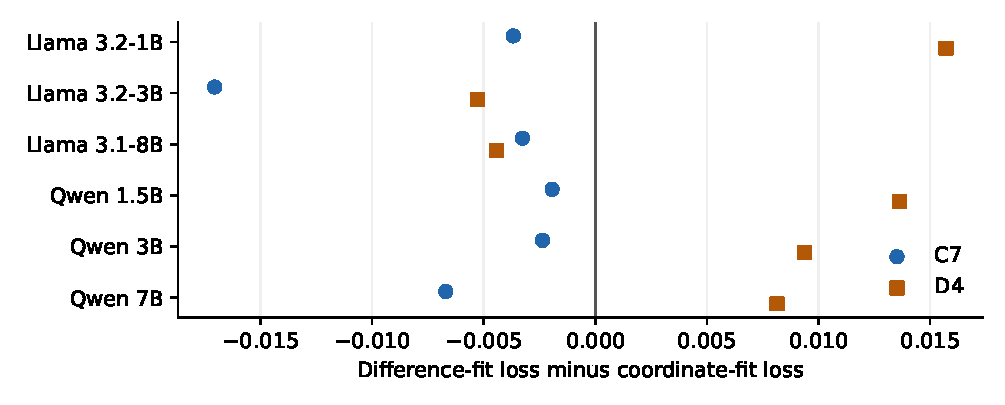
\includegraphics[width=.88\textwidth]{figures/context_transfer_followup.pdf}
\caption{New-context contrast by model and domain, averaging four fixed readouts. Negative values favor difference fitting. All six C7 model means are negative; D4 reverses direction in four models. Points are descriptive model means, not independent replications or confidence intervals. The primary aggregate and paired-family sensitivity ranges appear in \cref{tab:followup-context}.}
\label{fig:context-followup}
\end{figure}
The result narrows the original construction's finding: transport depends on the fitting objective, domain and language construction. The bank tests neither unseen state vocabulary nor arbitrary human prose; post-target text cannot affect a causal decoder's state-token readout. The family bootstrap preserves repeated cells and domains together and describes this authored bank, as specified in \cref{sec:setup}. No new significance, equivalence or native causal conclusion is drawn.
